\documentclass[11pt]{article}

\usepackage{graphicx}
\usepackage{amsthm}
\usepackage{listings}
\usepackage{fancyhdr}
\pagestyle{fancy}
\usepackage{indentfirst}
\usepackage{layout}
\usepackage{hanging}
\usepackage{setspace}
\usepackage{mathtools}

\DeclarePairedDelimiter\qb{\lvert}{\rangle}

\def\tit{Quantum Programming HW3}
\def\term{January 2020}

\graphicspath{{.}}

\def\auths{Joshua Larkin}


\doublespacing

\lhead{\term}
\chead{\tit}
\rhead{\thepage}
\cfoot{}


\title{
    \vspace{2in}
    \textmd{\textbf{\tit}}\\
    \normalsize\vspace{0.1in}\small{B490 : Spring 2020 }\\
    \vspace{0.1in}\large{\textit{\auths}}
    \vspace{3in}
}

\date{}

\newcommand{\icol}[1]{
  \left(\begin{smallmatrix}#1\end{smallmatrix}\right)
}


\newcommand{\n}{\newline}
\renewcommand\headrulewidth{0.4pt}
\fancyheadoffset{0.5 cm}

\oddsidemargin 0pt
\evensidemargin 0pt
\topmargin -.3in
\headsep 20pt
%\footskip 20pt
\textheight 8.5in
\textwidth 6.25in

\setlength\topmargin{0pt}
\addtolength\topmargin{-\headheight}
\addtolength\topmargin{-\headsep}
\setlength\oddsidemargin{0pt}
\setlength\textwidth{\paperwidth}
\addtolength\textwidth{-2in}
\setlength\textheight{\paperheight}
\addtolength\textheight{-2in}

\begin{document}

%%%% TITLE PAGE
\maketitle
\pagebreak

%%%%% First content Page
\section{Exercise 1}

\begin{enumerate}
\item[1.] Here is my diagram: M means 3-bit majority and U means 3-bit unmajority-and-add \\ 

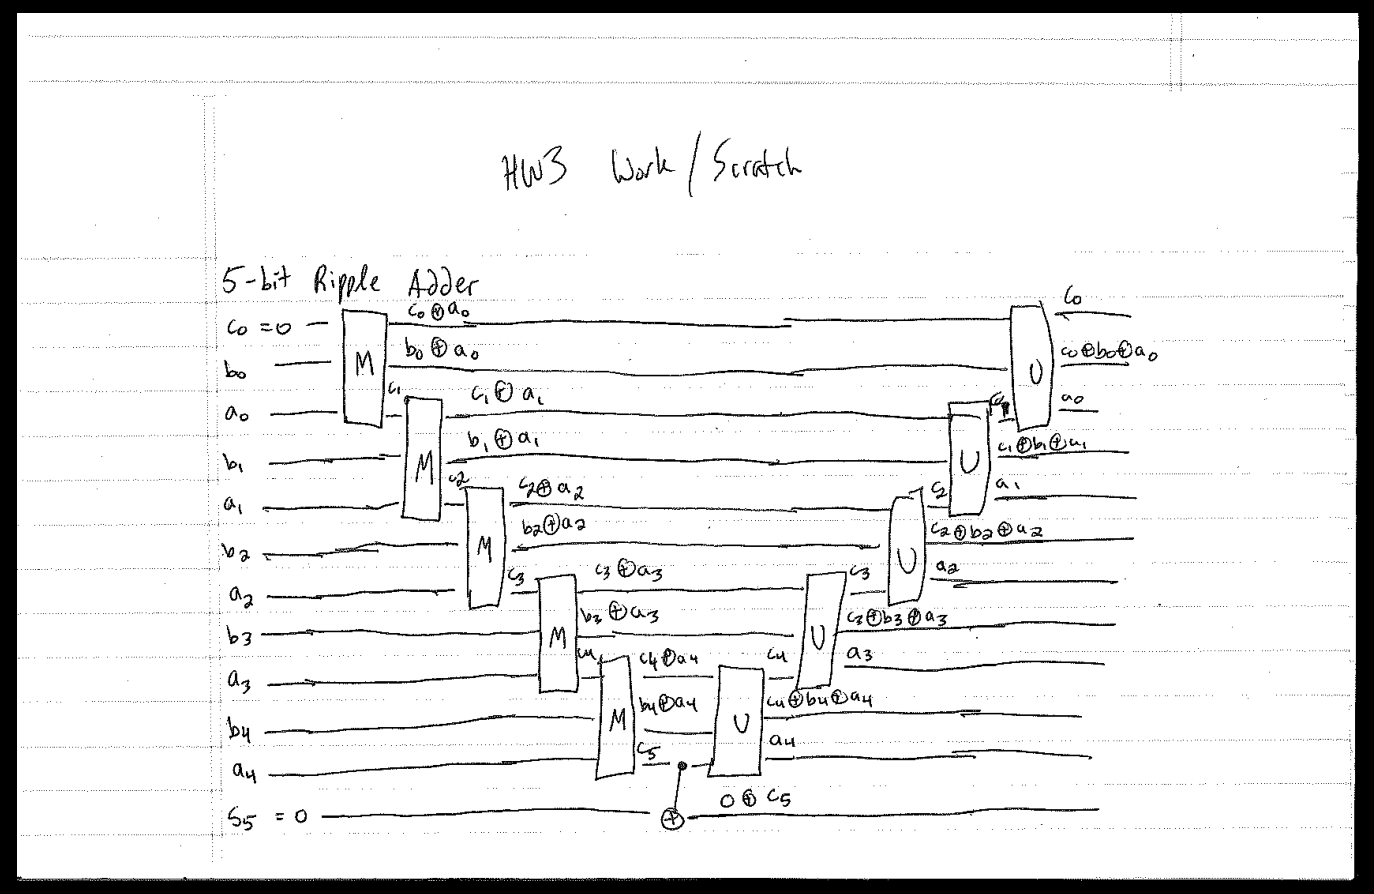
\includegraphics[width=\textwidth]{adder_img}


\item[2.] Included in a file titled $\texttt{adder\_n.txt}$

\item[3.] Included in a file titled $\texttt{adder.py}$ \\

\end{enumerate}

\newpage

\section{Exercise 2}

\begin{enumerate}

\item[1.] Convert the truth tables for the following functions/circuits into cyclic notation:
	For this, we will give each element of the given context set ($n$-bit) a unique letter,
		and the cycle notation for  transpositions of elements will use the letters.
	\begin{itemize}

	\item $x$ (in a 1-bit context) \\
	$x$ on $1$ bit is just $(a\ b)$ \\

	\begin{tabular}{c|c|c|c}
		$\_$ & $a$ & $x\ a$ & $\_$ \\
	\hline
		(a) & 0 & 1 & (b) \\
	\hline
		(b) & 1 & 0 & (a)
	\end{tabular}
	\vspace{.3in}
	\item $x$ (in a 4-bit context) \\
	The transposition here is $(a\ i) (b\ j) (c\ k) (d\ l) (e\ m) (f\ n) (g\ o) (h\ p)$ \\

	\begin{tabular}{c|c|c|c}
		$\_$ & $a$ & $x\ a$ & $\_$ \\
	\hline
		(a) & 0000 & 1000 & (i)  \\
	\hline                             
		(b) & 0001 & 1001 & (j)  \\
	\hline                             
		(c) & 0010 & 1010 & (k)  \\
	\hline                             
		(d) & 0011 & 1011 & (l)  \\
	\hline                             
		(e) & 0100 & 1100 & (m)  \\
	\hline                             
		(f) & 0101 & 1101 & (n)  \\
	\hline                             
		(g) & 0110 & 1110 & (o)  \\
	\hline                             
		(h) & 0111 & 1111 & (p)  \\
	\hline
	\end{tabular}
			\quad
	\begin{tabular}{c|c|c|c}
		$\_$ & $a$ & $x\ a$ & $\_$ \\
	\hline
	
		(i) & 1000 & 0000 & (a) \\ 
	\hline                             
		(j) & 1001 & 0001 & (b) \\ 
	\hline                             
		(k) & 1010 & 0010 & (c) \\ 
	\hline                             
		(l) & 1011 & 0011 & (d) \\ 
	\hline                             
		(m) & 1100 & 0100 & (e) \\ 
	\hline                             
		(n) & 1101 & 0101 & (f) \\ 
	\hline                             
		(o) & 1110 & 0110 & (g) \\ 
	\hline                             
		(p) & 1111 & 0111 & (h) \\ 
	\end{tabular}

	%% END X IN 4 BIT CONTEXT
	\newpage
	\item $cx$ (in a 2-bit context) \\
	The transposition is: $(c\ d)$  \\

	\begin{tabular}{c|c|c|c}
		$\_$ & $a$ & $cx\ a$ & $\_$ \\
	\hline
		(a) & 00 & 00 & (a) \\
	\hline
		(b) & 01 & 01 & (b) \\
	\hline 
		(c) & 10 & 11 & (d) \\
	\hline 
		(d) & 11 & 10 & (c) \\
	\end{tabular}


	\vspace{0.3in}
	%% END CX IN 2 BIT CONTEXT

	\item $cx$ (in a 4-bit context) \\
	The transposition is: $(i\ m) (j\ n) (k\ o) (l\ p)$  \\

	\begin{tabular}{c|c|c|c}
		$\_$ & $a$ & $cx\ a$ & $\_$ \\
		\hline (a) &  0000 &  0000 & (a) \\  
		\hline (b) &  0001 &  0001 & (b) \\ 
		\hline (c) &  0010 &  0010 & (c) \\ 
		\hline (d) &  0011 &  0011 & (d) \\ 
		\hline (e) &  0100 &  0100 & (e) \\ 
		\hline (f) &  0101 &  0101 & (f) \\ 
		\hline (g) &  0110 &  0110 & (g) \\ 
		\hline (h) &  0111 &  0111 & (h) \\ 
	\end{tabular}
	\quad\quad
	\begin{tabular}{c|c|c|c}
		$\_$ & $a$ & $cx\ a$ & $\_$ \\
		\hline (i) &  1000 &  1100 & (m) \\ 
		\hline (j) &  1001 &  1101 & (n) \\ 
		\hline (k) &  1010 &  1110 & (o) \\ 
		\hline (l) &  1011 &  1111 & (p) \\ 
		\hline (m) &  1100 &  1000 & (i) \\ 
		\hline (n) &  1101 &  1001 & (j) \\ 
		\hline (o) &  1110 &  1010 & (k) \\ 
		\hline (p) &  1111 &  1011 & (l)
	\end{tabular}

	\newpage
	%% END CX IN 4 BIT CONTEXT

	\item $ccx$ (in a 3-bit context) \\
	The transposition is: $(g\ h)$ 

	\begin{tabular}{c|c|c|c}
	$\_$ & $a$ & $cx\ a$ & $\_$ \\

		\hline (a) &  000 &  000 & (a) \\
		\hline (b) &  001 &  001 & (b) \\
		\hline (c) &  010 &  010 & (c) \\  
		\hline (d) &  011 &  011 & (d) \\ 
		\hline (e) &  100 &  100 & (e) \\ 
		\hline (f) &  101 &  101 & (f) \\ 
		\hline (g) &  110 &  110 & (h) \\ 
		\hline (h) &  111 &  111 & (g) 

	\end{tabular}

	\vspace{0.3in}
	%% END CCX IN 3 BIT CONTEXT

	\item $ccx$ (in a 4-bit context) \\
	The transposition is $(m\ o) (n\ p)$ 

	\begin{tabular}{c|c|c|c}
	$\_$ & $a$ & $cx\ a$ & $\_$ \\
\hline (a) &  0000 &  0000 & (a) \\ 
\hline (b) &  0001 &  0001 & (b) \\ 
\hline (c) &  0010 &  0010 & (c) \\ 
\hline (d) &  0011 &  0011 & (d) \\ 
\hline (e) &  0100 &  0100 & (e) \\ 
\hline (f) &  0101 &  0101 & (f) \\ 
\hline (g) &  0110 &  0110 & (g) \\ 
\hline (h) &  0111 &  0111 & (h) \\ 


	\end{tabular}
	\quad
	\begin{tabular}{c|c|c|c}
	$\_$ & $a$ & $cx\ a$ & $\_$ \\
\hline (i) &  1000 &  1000 & (i) \\ 
\hline (j) &  1001 &  1001 & (j) \\ 
\hline (k) &  1010 &  1010 & (k) \\ 
\hline (l) &  1011 &  1011 & (l) \\ 
\hline (m) &  1100 &  1110 & (o) \\ 
\hline (n) &  1101 &  1111 & (p) \\ 
\hline (o) &  1110 &  1100 & (m) \\ 
\hline (p) &  1111 &  1101 & (n) \\ 

	\end{tabular}
	\end{itemize}

	\newpage
	%% END CCX IN 4 BIT CONTEXT
\item[2.] Prove that the function CCCNOT cannot be implemented with a 4-bit circuit using the gate basis $\{\texttt{x}, \texttt{cx}, \texttt{ccx} \}$
\begin{proof}
	We know from our above work that each of the gates, in a 4-bit context, are transpositions of even parity. 
	By the given theorem, we know that any composition of the gates in the gate basis will have an even length. 
	Consider the CCCNOT function: it will swap 1110 and 1111, and leave all other inputs fixed. This means that CCCNOT is essentially a transposition of odd parity. 
	Hence we cannot implement CCCNOT using the gate basis 
	$\{\texttt{x}, \texttt{cx}, \texttt{ccx} \}$
\end{proof}


\item[3.] Prove that a 5-bit majority function cannot be implemented with a 5-bit circuit
	using the gate basis $\{\texttt{x}, \texttt{cx}, \texttt{ccx} \}$
\begin{proof}
	We claim that the basis gates are still transpositions of even parity in a 5-bit context. 
	In the case for $\texttt{x}$, we will swap all 32 rows, which is 16 transpositions. 
	In the case for $\texttt{cx}$, we will swap 16 rows, which is 8 transpositions. 
	In the case for $\texttt{ccx}$ we will swap 8 rows, which is 4 transpositions. 
	We claim that the majority function has 10 row swaps, and is thus a 5 transposition function.
	The majority function will have one of the bits represent the majority, 
		so there will be some column of the output that has a 1 when there is a majority. 
	We may assume without loss of generality that this is the first column of the output. 
	Of the first 16 rows of possible inputs, there are 5 that will need to be swapped: 
	00111, 01011, 01101, 01110, 01111.
	And becaues of the symmetry of  5 bits, there will be 5 more in the last 16 rows.
	So we know majority is a odd parity transposition function, 
	    and our gate basis is only made up of even parity transposition functions, 
	    so there is no way to implement majority with the gate basis 
	    $\{\texttt{x}, \texttt{cx}, \texttt{ccx} \}$
\end{proof}

\end{enumerate}

\newpage

\section{Exercise 3} Define $\texttt{toffoli}(n)$ in $\Pi$.
\begin{lstlisting}
tof :: (n : Nat) -> B^n <-> B^n
tof 0     = id
tof 1     = not
tof 2     = distrib; ((id x not) + id); factor
tof n + 1 = distrib; (tof n); factor
\end{lstlisting}

\section{Exercise 4} Define $\texttt{toffoli}(n)$ in Thesus.
First recall these definition from Theseus:
\begin{lstlisting}
not :: Bool <-> Bool
| True  <-> False
| False <-> True

if :: th:(a <-> a) -> el:(a <-> a) -> Bool x a <-> Bool x a
| True,  a <-> True, th a
| False, a <-> False, el a

cx :: Bool x Bool <-> Bool x Bool
| x <-> if ~th:not ~el:id x
\end{lstlisting}

Now we can define Toffoli:
\begin{lstlisting}
tof :: (n : Nat) -> B^n <-> B^n
| 0     <-> id
| 1     <-> not
| 2     <-> cx
| n + 1 <-> if ~th:(tof n) ~el:id 
\end{lstlisting}



\end{document}
